\documentclass{beamer}
\mode<presentation>
{
	\usetheme{Berkeley}
	\usecolortheme{default}
	\usefonttheme{default}
	\setbeamertemplate{navigation symbols}{}
	\setbeamertemplate{caption}[numbered]
}

\usepackage{listings}
\usepackage[english]{babel}
\usepackage[utf8x]{inputenc}

\title[SHARE]{SHARE}
\author{Erik Schilling\\Philipp	Ostmeyer}
\institute{Universität Paderborn}
\date{4th of October 2016}

\begin{document}

	\section{}
	\begin{frame}
		\titlepage
	\end{frame}

	\section{Content}
	\subsection{Introduction}
	\begin{frame}{Introduction}
		\begin{block}{SHARE}
			\begin{itemize}
				\item Non-uniform Storage-Nodes
				\item Distributed storage of data
				\item Server driven
			\end{itemize}
		\end{block}

		\begin{itemize}
			\item Allows nodes with different capacities
			\item Each node has a interval depending on the capacity
			\item Two-level hashing
			\begin{itemize}
				\item One hash function maps data to an id section
				\item Second hash function maps from data to a storage node in this id section
			\end{itemize}
		\end{itemize}
	\end{frame}
	\subsection{Architecture}
	\begin{frame}{Solution}
		\begin{block}{Logic}
			\begin{itemize}
				\item Internally based on Subject class from exercises
				\item Websocket server implemented with Java-Websocket\footnote{\url{https://github.com/TooTallNate/Java-WebSocket}}
				\item Serialisation with Gson\footnote{\url{https://github.com/google/gson}}
			\end{itemize}
		\end{block}
		\begin{block}{UI}
			\begin{itemize}
				\item Web based UI
				\item Implemented with Angular 2\footnote{\url{https://angular.io/}}
				\item Written in TypeScript
			\end{itemize}
		\end{block}
	\end{frame}
	\begin{frame}{Architecture}
		\begin{figure}
			\hspace{0.1cm}
			\raggedright
			\begin{minipage}{1cm}
				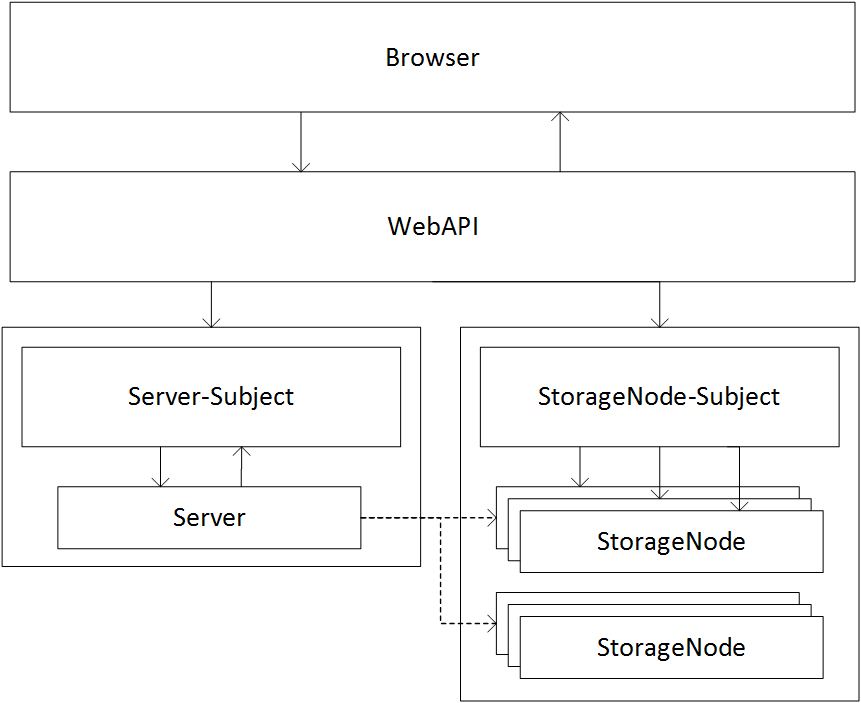
\includegraphics[width=9cm]{architecture.png}
			\end{minipage}
		\end{figure}
	\end{frame}
	\subsection{Message-Pathing}
	\begin{frame}{Message-Pathing}
		\begin{figure}
			\raggedright
			\begin{minipage}{1cm}
				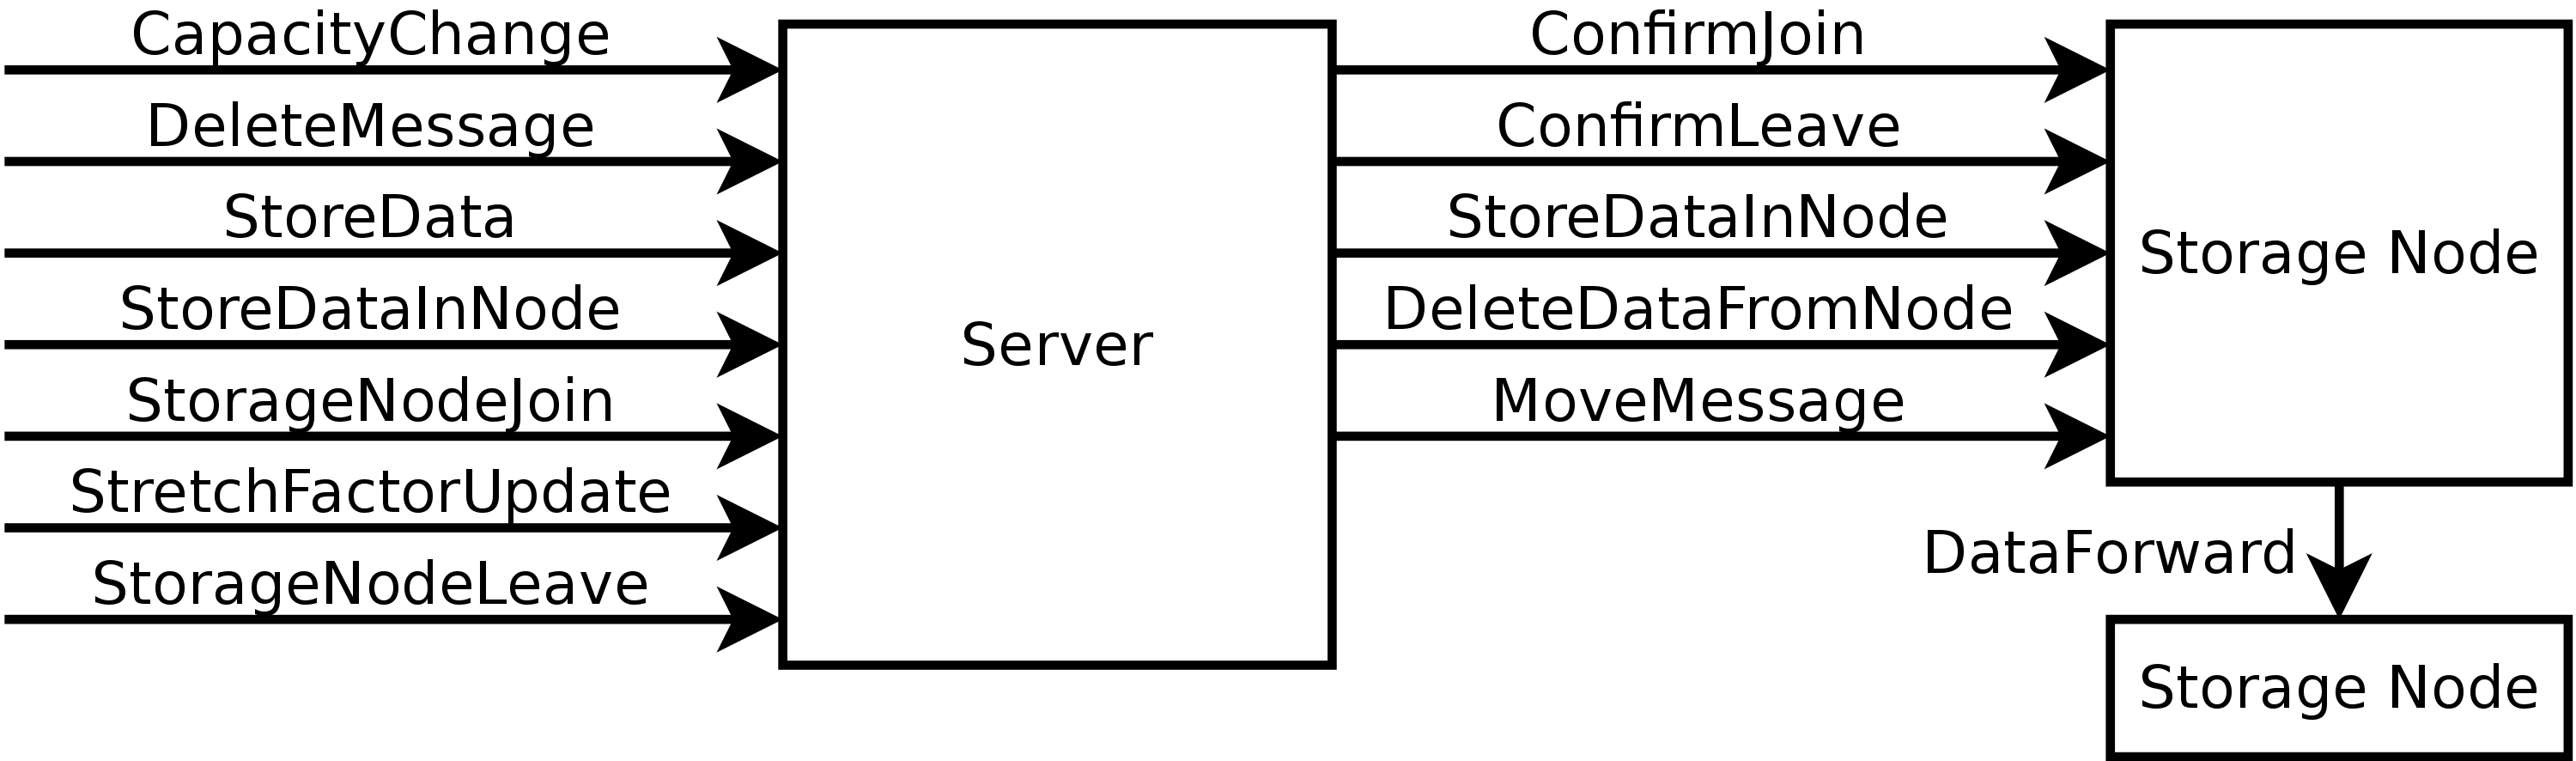
\includegraphics[width=10cm]{messages.png}
			\end{minipage}
		\end{figure}
	\end{frame}
	\subsection{Demo}
	\begin{frame}{Demo}
		\begin{figure}
			\raggedright
			\begin{minipage}{1cm}
				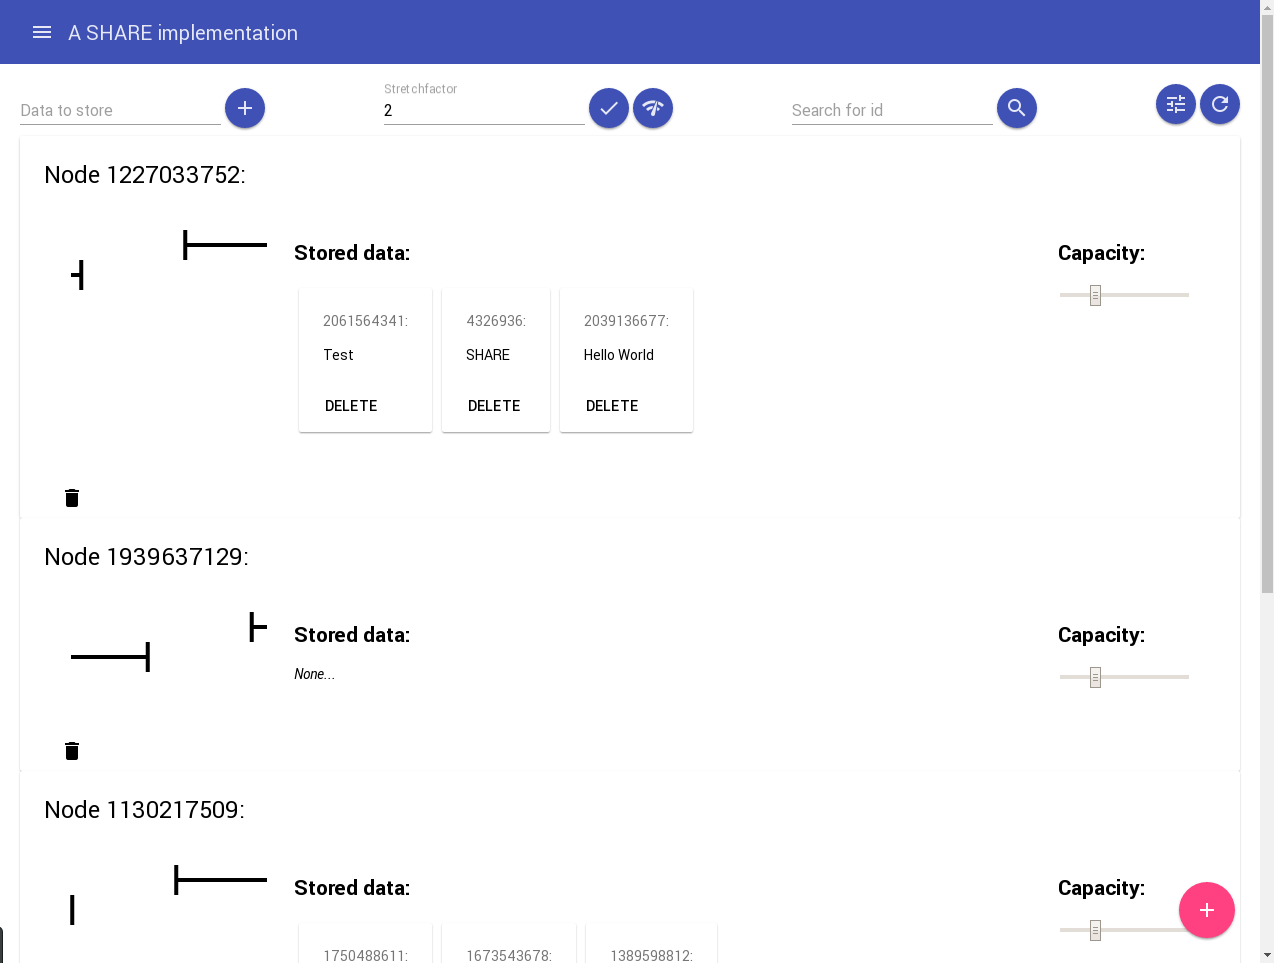
\includegraphics[width=10cm]{app.png}
			\end{minipage}
		\end{figure}
	\end{frame}

\end{document}
